\chapter{Server}
\section{Virtual Machine}

During the development of the BMONS systems, we opted for the utilization of a Virtual Machine. A virtual machine is a way to emulate a particular computer system from another system. Considering that most of the development would take place during class and inside the school's labs, we are faced with one issue: not having full administrator powers and full control of the software we are allowed to install. Having a complete virtual machine also allows a full portability of our development environment since it's common that the actual physical machines used for development vary between classes. Another advantage includes reducing the stress of deployment and developing in a safe environment. Once the project is done, it is possible to just copy the virtual machine to its final destination instead of doing a full reinstall of the system. Should any problems occur during the development, like corruption of the essential packages, for example, it will not affect the main system from which the virtual machine is loaded. Multiple virtual machines can co-exist in a hard drive, each one having its own full environment, using different softwares installed and eliminating possible conflicts. Even though a virtual is somewhat "closed", it is possible to share files between the main system (host) and a virtual machine (guest) using specific partitions. 

By using the software called Oracle VM VirtualBox, we were able to create a full development environment in a virtual machine with the Ubuntu operational system version 14.04. Ubuntu was our choice of operational system because it combines the power and possibilities of a Unix system, useful packages installed out of the box and a friendly Graphical User Interface. All that while still being completely free to use, since Ubuntu is an open source software. 

Once the operational system is installed on the virtual machine, it might be necessary to configure a network proxy so it is possible to access the internet from within. That is the case when using computers from the school's labs. Using Ubuntu, however, this is not such a difficult task. A proxy can be added by accessing System's Settings > Network > Proxy. 

\clearpage
\begin{figure}[h]
\centering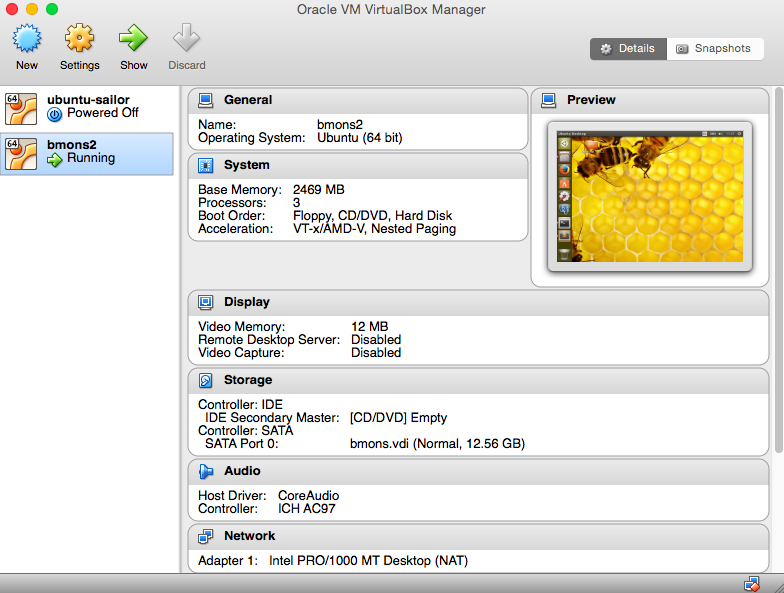
\includegraphics[scale=0.5]{virtualbox.png}
\caption{\label{fig:virtualbox} Oracle VM VirtualBox Software}
\end{figure}

\begin{figure}[h]
\centering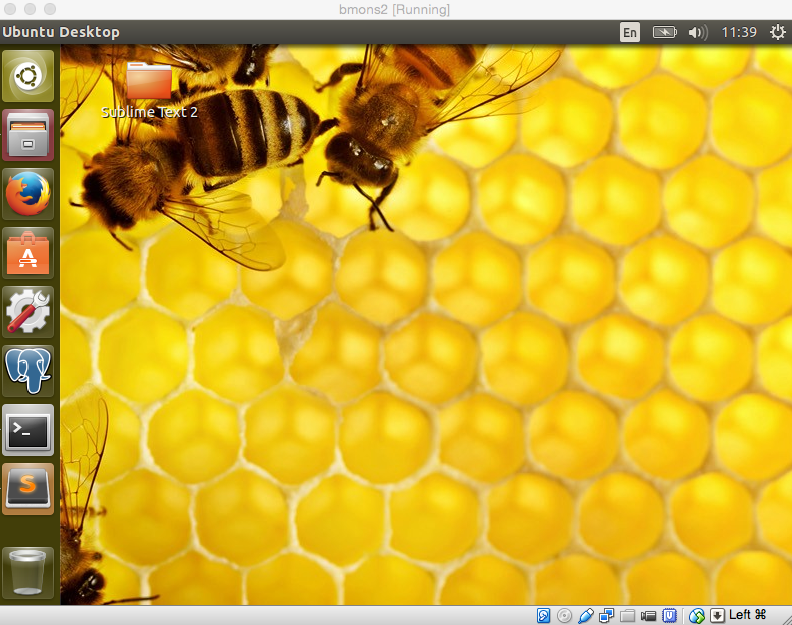
\includegraphics[scale=0.5]{ubuntu.png}
\caption{\label{fig:ubuntu} Ubuntu 14.04 loaded from Oracle VM Virtual Box}
\end{figure}

\clearpage

\section{Basic packages and installation}

To install BMONS on the virtual machine, it is firstly necessary either to download BMONS from the github repository located at https://github.com/Etiene/sailor/archive/master.zip or to download at least the file called install.sh, located at the directory /scripts/server.

Even though a virtual machine allows a portable environment, eliminating the need to install all software needed everytime a developer changes computers, sometimes errors might occur and a fresh install of the system might be necessary. This is why BMONS is provided with a install script for the server side. A bash script, extension .sh, runs multiple commands that normally would be necessary to be ran in the command line terminal and is very useful for automating tasks or a repeated sequence of commands. The install.sh file provided with BMONS will, then, automatically install most of the required software to run the BMONS server and modify it. Please note that this script should be run by the root user or using the privileges of the root user by using sudo.

\indent cd <location of BMONS at the filesystem>/scripts/server
\indent sudo ./install.sh

Among the essential packages installed by this script you will find: Git, the version control software used to keep track of BMONS; Ruby, the server-side programming language used on BMONS's website; Rails - the framework over which BMONS's website is developed; PostgreSQL - the database used to store BMONS's data; and pgAdmin III - a GUI (Graphical User Interface) software to administrate PostgreSQL.

An IDE (Integrated Development Environment) is not provided with the install script. Not only some IDEs are needlessly heavy, we believe that each developer has the right to choose their preferred way to write their code. The choice of our team was to use regular text editors, like gedit or Sublime Text (recommended).

\clearpage
\section{Webserver}

BMONS's website's server files are located under the directory bmons-site of our files. 

Before the first use of BMONS, it is necessary to navigate to this directory and run 'bundle install' and 'rake db:schema:load' at the command line. Please note that this step is not necessary if you are running BMONS from a previously configured virtual machine. This is required only if it is a fresh install of BMONS and only before the first time of running the webserver.

\indent cd <location of BMONS at the filesystem>/bmons-site
\indent bundle install
\indent rake db:schema:load

BMON's website uses some third-party softwares that made the development phase more productive, such as Devise, for example. Devise is a full-featured authentication solution which handles all of the controller logic and form views. This was used to implement the login system for BMONS. Running 'bundle install' will install all the necessary gems (plugins for the Ruby language) required to run Rails and the other gems that we chose to use during development. 

When installing the server for the first time, the database will be empty. It will not contain the tables that store our data. This is why the command 'rake db:schema:load' is necessary. It will load the schema of the entities used by the website and generate the queries that will create those tables.

To start the server, it is necessary to run the command 'rails server'.

\indent cd <location of BMONS at the filesystem>/bmons-site
\indent rails server

Once that is done, the website will be accessible via the url configured.

\clearpage
\section{Database and Backup}

The choice of database our team made for BMONS was PostgreSQL. Many options were possible but there are some advantages to using this specific one. While NoSQL databases are interesting and can be very fast in terms of performance, they are not very easy to deal in terms of development. Also, NoSQL is usually very fast for accessing and reading data but not so fast for writing and inserting data. Normally, BMONS should insert data way more frequently than reading. That is because one single user that is not connected to the website the whole time can have multiple beehives that will be sending data to the server on a regular basis, making us to reject this option right away. In addition to this, the archirecture of BMONS's data is already compatible with a regular SQL relational data.

There are many possible options of SQL databases, however, among those, PostgreSQL was favored because our team already had some knowledge of it and because it is a very good, reliable and stable open source software that is capable of dealing with very high volumes of data if necessary.

It is recommended to do database backups regularly. In case data is corrupted, it will be possible to restore the original data from recent a backup. BMONS is provided with a script that will automatically dump the database data into a dated file in the filesystem regularly (every 3 hours). It is recommended that that these generated files are copied to a safe location, such as another computer or an external hard drive from time to time.

Cron is an automatic scheduler for Unix systems that will run command line commands in specific times or time intervals according to the following pattern:
  #comment
  * * * * *  command to execute
  │ │ │ │ │
  │ │ │ │ │
  │ │ │ │ └───── day of week (0 - 6)
  │ │ │ └────────── month (1 - 12)
  │ │ └─────────────── day of month (1 - 31)
  │ └──────────────────── hour (0 - 23)
  └───────────────────────── min (0 - 59)

To activate the automatic backups, it is necessary to navigate to the directory /scripts/server of BMONS files. Under this directory is located a file called cron.txt. When making a fresh install of BMONS, it might be necessary to edit the line 6 of this file and correct the path to the backup bash script. It is also possible to change the frequency of the backups if desired. 
 
\texttt{0 */3 * * * /home/bmons/BMONS/scripts/server/db\_backup.sh}

Then you can run the following command to incorporate this cron job into the schedule:

\indent crontab cron.txt

\clearpage
\section{The web interface}

The web interface of BMONS was built using Ruby on Rails. Rails is an open source web application development framework written in the Ruby language. It's used specially for developing database-driven websites and allows the creation of applications using pre defined structures. Rails is a Model-View-Controller (MVC) framework. MVC is a software design pattern for implementing user interfaces. It divides the software into three interconnected parts. 
Models: They store the data of the application, its business rules and methods. It's often regarded as a "mirror" of the database.
Views: They're the output of a model data representation, such as a table or a diagram, for the user.
Controllers: They make the mediation between the models and the views, sending commands to update models' states and sending commands to the view to alter the presentation of the models.

The Rails philosophy includes two major guiding principles:

"Don't Repeat Yourself: DRY is a principle of software development which states that "Every piece of knowledge must have a single, unambiguous, authoritative representation within a system." By not writing the same information over and over again, our code is more maintainable, more extensible, and less buggy.
Convention Over Configuration: Rails has opinions about the best way to do many things in a web application, and defaults to this set of conventions, rather than require that you specify every minutiae through endless configuration files."

Rails philosophy and features allowed our team to develop an interesting application in a feasible time. This web application allows a beekeeper to register, login, change password, see a dashboard with visual data from their hives and manage hives and alerts. The application will also receive content from the Arduino located at the hive and update its data.

The authentication system was developed with the use of Devise, which is a plugin that fully handles the authentication through the MVC pattern. The pages to manage beehives, sensors, measurements, alerts and alert logs were firstly created with the use of scaffolding. A scaffold in Rails is a full set of model, database migration for that model, controller to manipulate it, views to view and manipulate the data, and a test suite for each of the above. This scaffold can be created through the command line in a very easy manner.

rails generate scaffold Beehive name:string user:references position:string mode:string

However, scaffolding alone is not enough and after the creation it is necessary to rearrange and modify the code to make it suit our needs. One example is modifying the beehive scaffold for showing only the beehives that belong to the user currently logged in.

One important aspect of the BMONS's website is the design. The design was developed with the help of Bootstrap. Bootstrap is a free and open source front-end framework that uses HTML, CSS, and JavaScript to provide re-usable components and other interface elements. It allows the development of responsive and mobile first projects on the web. With some customization Bootstrap, we were able to obtain pages that display our system's contents beautifully. We opted for changing the color palette into a yellow
and dark gray theme on a light background because it's aesthetically beautiful, readable and refers well to a bee's color pattern.

Bootstrap, however, is not enough for displaying our data. The dashboard requires the data to be easily grasped and even though tables are really useful, they are not sufficient to provide a quick visual analysis. Our team's choice of optimal display was a graphical one. The development of the graphical dashboard was made with NVD3, a JavaScript library that extends another library called D3 that allows you to bind arbitrary data to a Document Object Model (DOM), and then apply data-driven transformations to the document. The advantage of using NVD3 over D3 is that it is an easier to use library with a reduced collection of components that satisfies our needs without taking away the power of D3. The data is then passed from the controller backend in ruby to the frontend view in a JavaScript piece of code that is then used and manipulated by the NVD3 library, producing beautiful results. The graphic allows for the visualization of measures from sensors in time of each individual beehive, allowing to switch between hives without refreshing the page. 

\clearpage
\begin{figure}[h]
\centering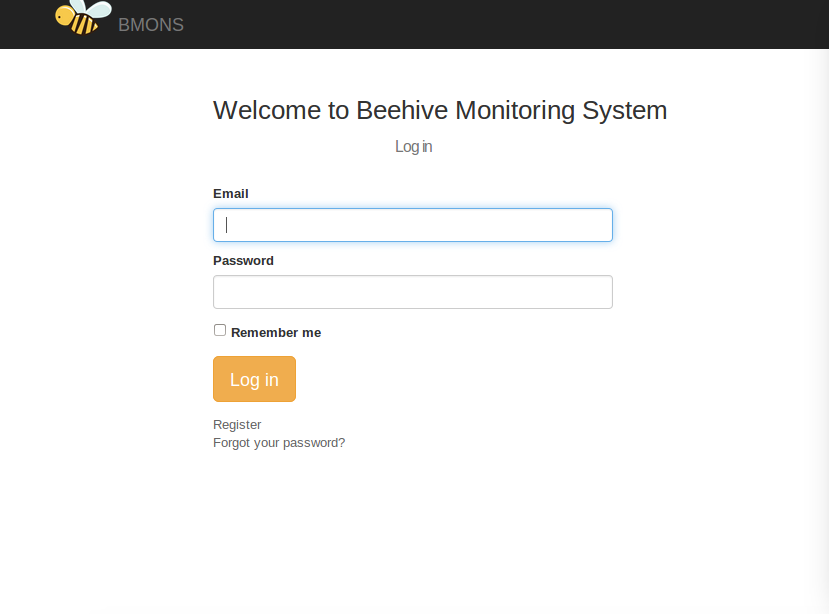
\includegraphics[scale=0.5]{login.png}
\caption{\label{fig:login} Initial page of BMONS web page. User authentication is necessary. }
\end{figure}

\begin{figure}[h]
\centering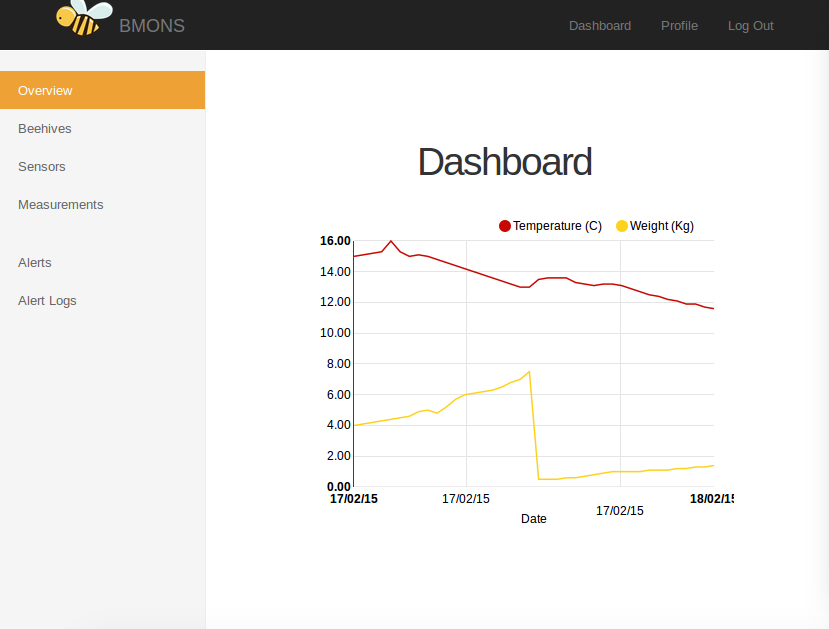
\includegraphics[scale=0.5]{dashboard.png}
\caption{\label{fig:dashboard} The initial page once the user is logged in shows the dashboard. }
\end{figure}

\begin{figure}[h]
\centering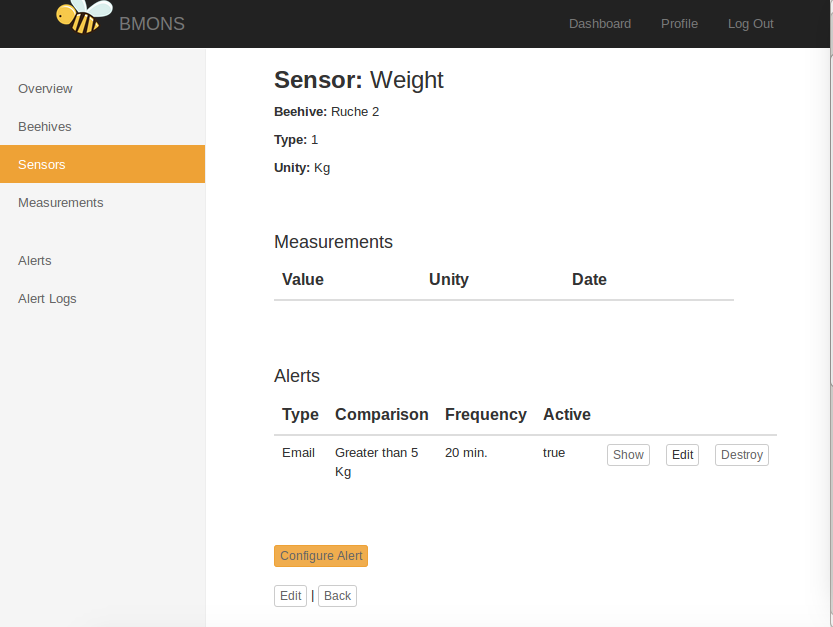
\includegraphics[scale=0.5]{sensor.png}
\caption{\label{fig:sensor} Page that shows a sensor information }
\end{figure}

\begin{figure}[h]
\centering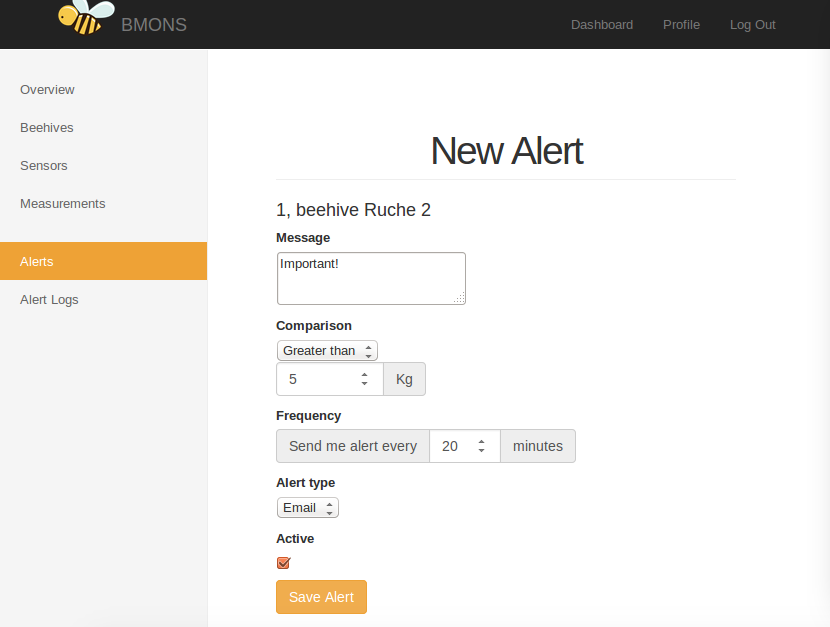
\includegraphics[scale=0.5]{alert.png}
\caption{\label{fig:alert} Page to create a new alert. }
\end{figure}

\clearpage

\section{The API and receipt of data from external source}

BMONS contains an API for receiving the captured data by the Arduino and storing it on a database for later displaying to the beekeeper. By default a Ruby on Rails CRUD (create, read, update and delete actions for an entity) is already a REST (Representational State Transfer) API that will perform the necessary actions using the right HTTP protocol request method and with full JSON capability. A PATCH or PUT will access the update action, a GET will obtain the data in a JSON object as a response, a DELETE will access the delete action and destroy the desired data and, finally, a POST will receive a JSON object and store new data. For BMONS needs, it was necessary to use the POST request to receive new measurements periodically from an external source, the Arduino, instead of from a form in a view used by an authenticated user. To make sure the data coming in is still safe, for the measurement create action, instead of a user authentication, a Basic HTTP Authentication is used. That means that the POST request sent by the Arduino must also send an authentication token on its header and the data will only be stored if the details are correct. In addition to the authentication, the Arduino must also sent, of course, the data. The content-type of this request should be application/JSON and a JSON object containing the necessary information for creating a new measurement should be included in the body of the request. To test BMONS's RESTful API, a browser extension named Postman was used as a client. 
